\documentclass[twoside]{book}

% Packages required by doxygen
\usepackage{calc}
\usepackage{doxygen}
\usepackage{graphicx}
\usepackage[utf8]{inputenc}
\usepackage{makeidx}
\usepackage{multicol}
\usepackage{multirow}
\usepackage{textcomp}
\usepackage[table]{xcolor}

% Font selection
\usepackage[T1]{fontenc}
\usepackage{mathptmx}
\usepackage[scaled=.90]{helvet}
\usepackage{courier}
\usepackage{amssymb}
\usepackage{sectsty}
\renewcommand{\familydefault}{\sfdefault}
\allsectionsfont{%
  \fontseries{bc}\selectfont%
  \color{darkgray}%
}
\renewcommand{\DoxyLabelFont}{%
  \fontseries{bc}\selectfont%
  \color{darkgray}%
}

% Page & text layout
\usepackage{geometry}
\geometry{%
  a4paper,%
  top=2.5cm,%
  bottom=2.5cm,%
  left=2.5cm,%
  right=2.5cm%
}
\tolerance=750
\hfuzz=15pt
\hbadness=750
\setlength{\emergencystretch}{15pt}
\setlength{\parindent}{0cm}
\setlength{\parskip}{0.2cm}
\makeatletter
\renewcommand{\paragraph}{%
  \@startsection{paragraph}{4}{0ex}{-1.0ex}{1.0ex}{%
    \normalfont\normalsize\bfseries\SS@parafont%
  }%
}
\renewcommand{\subparagraph}{%
  \@startsection{subparagraph}{5}{0ex}{-1.0ex}{1.0ex}{%
    \normalfont\normalsize\bfseries\SS@subparafont%
  }%
}
\makeatother

% Headers & footers
\usepackage{fancyhdr}
\pagestyle{fancyplain}
\fancyhead[LE]{\fancyplain{}{\bfseries\thepage}}
\fancyhead[CE]{\fancyplain{}{}}
\fancyhead[RE]{\fancyplain{}{\bfseries\leftmark}}
\fancyhead[LO]{\fancyplain{}{\bfseries\rightmark}}
\fancyhead[CO]{\fancyplain{}{}}
\fancyhead[RO]{\fancyplain{}{\bfseries\thepage}}
\fancyfoot[LE]{\fancyplain{}{}}
\fancyfoot[CE]{\fancyplain{}{}}
\fancyfoot[RE]{\fancyplain{}{\bfseries\scriptsize Generated on Wed Sep 30 2015 02\-:12\-:18 for My Project by Doxygen }}
\fancyfoot[LO]{\fancyplain{}{\bfseries\scriptsize Generated on Wed Sep 30 2015 02\-:12\-:18 for My Project by Doxygen }}
\fancyfoot[CO]{\fancyplain{}{}}
\fancyfoot[RO]{\fancyplain{}{}}
\renewcommand{\footrulewidth}{0.4pt}
\renewcommand{\chaptermark}[1]{%
  \markboth{#1}{}%
}
\renewcommand{\sectionmark}[1]{%
  \markright{\thesection\ #1}%
}

% Indices & bibliography
\usepackage{natbib}
\usepackage[titles]{tocloft}
\setcounter{tocdepth}{3}
\setcounter{secnumdepth}{5}
\makeindex

% Hyperlinks (required, but should be loaded last)
\usepackage{ifpdf}
\ifpdf
  \usepackage[pdftex,pagebackref=true]{hyperref}
\else
  \usepackage[ps2pdf,pagebackref=true]{hyperref}
\fi
\hypersetup{%
  colorlinks=true,%
  linkcolor=blue,%
  citecolor=blue,%
  unicode%
}

% Custom commands
\newcommand{\clearemptydoublepage}{%
  \newpage{\pagestyle{empty}\cleardoublepage}%
}


%===== C O N T E N T S =====

\begin{document}

% Titlepage & ToC
\hypersetup{pageanchor=false}
\pagenumbering{roman}
\begin{titlepage}
\vspace*{7cm}
\begin{center}%
{\Large My Project }\\
\vspace*{1cm}
{\large Generated by Doxygen 1.8.6}\\
\vspace*{0.5cm}
{\small Wed Sep 30 2015 02:12:18}\\
\end{center}
\end{titlepage}
\clearemptydoublepage
\tableofcontents
\clearemptydoublepage
\pagenumbering{arabic}
\hypersetup{pageanchor=true}

%--- Begin generated contents ---
\chapter{Namespace Index}
\section{Namespace List}
Here is a list of all namespaces with brief descriptions\-:\begin{DoxyCompactList}
\item\contentsline{section}{\hyperlink{namespacevideorentalsystem}{videorentalsystem} }{\pageref{namespacevideorentalsystem}}{}
\end{DoxyCompactList}

\chapter{Hierarchical Index}
\section{Class Hierarchy}
This inheritance list is sorted roughly, but not completely, alphabetically\-:\begin{DoxyCompactList}
\item \contentsline{section}{carcruisecontrolsystem.\-Car\-Cruise\-Control\-System}{\pageref{classcarcruisecontrolsystem_1_1CarCruiseControlSystem}}{}
\item J\-Frame\begin{DoxyCompactList}
\item \contentsline{section}{carcruisecontrolsystem.\-Control}{\pageref{classcarcruisecontrolsystem_1_1Control}}{}
\item \contentsline{section}{carcruisecontrolsystem.\-Greeter}{\pageref{classcarcruisecontrolsystem_1_1Greeter}}{}
\end{DoxyCompactList}
\end{DoxyCompactList}

\chapter{Class Index}
\section{Class List}
Here are the classes, structs, unions and interfaces with brief descriptions\-:\begin{DoxyCompactList}
\item\contentsline{section}{\hyperlink{classcarcruisecontrolsystem_1_1CarCruiseControlSystem}{carcruisecontrolsystem.\-Car\-Cruise\-Control\-System} }{\pageref{classcarcruisecontrolsystem_1_1CarCruiseControlSystem}}{}
\item\contentsline{section}{\hyperlink{classcarcruisecontrolsystem_1_1Control}{carcruisecontrolsystem.\-Control} }{\pageref{classcarcruisecontrolsystem_1_1Control}}{}
\item\contentsline{section}{\hyperlink{classcarcruisecontrolsystem_1_1Greeter}{carcruisecontrolsystem.\-Greeter} }{\pageref{classcarcruisecontrolsystem_1_1Greeter}}{}
\end{DoxyCompactList}

\chapter{File Index}
\section{File List}
Here is a list of all files with brief descriptions\-:\begin{DoxyCompactList}
\item\contentsline{section}{\hyperlink{CostData_8java}{Cost\-Data.\-java} }{\pageref{CostData_8java}}{}
\item\contentsline{section}{\hyperlink{Costumer_8java}{Costumer.\-java} }{\pageref{Costumer_8java}}{}
\item\contentsline{section}{\hyperlink{CostumerForm_8java}{Costumer\-Form.\-java} }{\pageref{CostumerForm_8java}}{}
\item\contentsline{section}{\hyperlink{Movie_8java}{Movie.\-java} }{\pageref{Movie_8java}}{}
\item\contentsline{section}{\hyperlink{Producer_8java}{Producer.\-java} }{\pageref{Producer_8java}}{}
\item\contentsline{section}{\hyperlink{Rental_8java}{Rental.\-java} }{\pageref{Rental_8java}}{}
\item\contentsline{section}{\hyperlink{RentVideo_8java}{Rent\-Video.\-java} }{\pageref{RentVideo_8java}}{}
\item\contentsline{section}{\hyperlink{VideoData_8java}{Video\-Data.\-java} }{\pageref{VideoData_8java}}{}
\item\contentsline{section}{\hyperlink{VideoForm_8java}{Video\-Form.\-java} }{\pageref{VideoForm_8java}}{}
\item\contentsline{section}{\hyperlink{VideoRentalSystem_8java}{Video\-Rental\-System.\-java} }{\pageref{VideoRentalSystem_8java}}{}
\item\contentsline{section}{\hyperlink{Welcome_8java}{Welcome.\-java} }{\pageref{Welcome_8java}}{}
\end{DoxyCompactList}

\chapter{Namespace Documentation}
\hypertarget{namespaceiikh}{\section{Package iikh}
\label{namespaceiikh}\index{iikh@{iikh}}
}
\subsection*{Classes}
\begin{DoxyCompactItemize}
\item 
class \hyperlink{classiikh_1_1Database}{Database}
\item 
class \hyperlink{classiikh_1_1Greeter}{Greeter}
\item 
class \hyperlink{classiikh_1_1IIKH}{I\-I\-K\-H}
\item 
class \hyperlink{classiikh_1_1MealData}{Meal\-Data}
\item 
class \hyperlink{classiikh_1_1MealManager}{Meal\-Manager}
\item 
class \hyperlink{classiikh_1_1PlanData}{Plan\-Data}
\item 
class \hyperlink{classiikh_1_1PlanManager}{Plan\-Manager}
\item 
class \hyperlink{classiikh_1_1RecipeForm}{Recipe\-Form}
\end{DoxyCompactItemize}

\chapter{Class Documentation}
\hypertarget{classiikh_1_1Database}{\section{iikh.\-Database Class Reference}
\label{classiikh_1_1Database}\index{iikh.\-Database@{iikh.\-Database}}
}


Collaboration diagram for iikh.\-Database\-:
\nopagebreak
\begin{figure}[H]
\begin{center}
\leavevmode
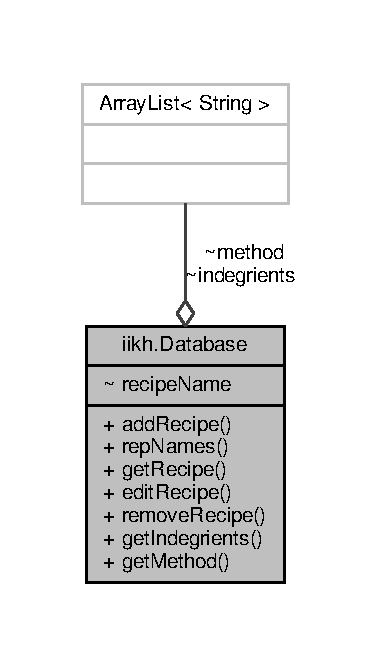
\includegraphics[width=183pt]{classiikh_1_1Database__coll__graph}
\end{center}
\end{figure}
\subsection*{Public Member Functions}
\begin{DoxyCompactItemize}
\item 
void \hyperlink{classiikh_1_1Database_a3126cde12781a55dfc8898452843aca5}{add\-Recipe} (String recipe\-Name, Array\-List$<$ String $>$ indegrients, Array\-List$<$ String $>$ method)
\item 
Array\-List$<$ String $>$ \hyperlink{classiikh_1_1Database_a3cae2850a17856de5310e386d6d0a496}{rep\-Names} ()
\item 
void \hyperlink{classiikh_1_1Database_a0515f744922af9d3cef297a3d66fcecc}{get\-Recipe} (String recipe\-Name)
\item 
void \hyperlink{classiikh_1_1Database_a60b7b747492c6ef9dd01632750b817f3}{edit\-Recipe} (String old\-Recipe\-Name, String new\-Recipe\-Name, Array\-List$<$ String $>$ indegrients, Array\-List$<$ String $>$ method)
\item 
void \hyperlink{classiikh_1_1Database_ae511be60eac7e23f273b4afcb92ec7b7}{remove\-Recipe} (String Recipe\-Name)
\item 
Array\-List$<$ String $>$ \hyperlink{classiikh_1_1Database_a17e77feed3e9e1ac003aded0d9a449a8}{get\-Indegrients} ()
\item 
Array\-List$<$ String $>$ \hyperlink{classiikh_1_1Database_a3a7aeca4a1ed5e510a8801a389e28e29}{get\-Method} ()
\end{DoxyCompactItemize}


\subsection{Detailed Description}
\begin{DoxyAuthor}{Author}
oop31 
\end{DoxyAuthor}


\subsection{Member Function Documentation}
\hypertarget{classiikh_1_1Database_a3126cde12781a55dfc8898452843aca5}{\index{iikh\-::\-Database@{iikh\-::\-Database}!add\-Recipe@{add\-Recipe}}
\index{add\-Recipe@{add\-Recipe}!iikh::Database@{iikh\-::\-Database}}
\subsubsection[{add\-Recipe}]{\setlength{\rightskip}{0pt plus 5cm}void iikh.\-Database.\-add\-Recipe (
\begin{DoxyParamCaption}
\item[{String}]{recipe\-Name, }
\item[{Array\-List$<$ String $>$}]{indegrients, }
\item[{Array\-List$<$ String $>$}]{method}
\end{DoxyParamCaption}
)\hspace{0.3cm}{\ttfamily [inline]}}}\label{classiikh_1_1Database_a3126cde12781a55dfc8898452843aca5}
\hypertarget{classiikh_1_1Database_a60b7b747492c6ef9dd01632750b817f3}{\index{iikh\-::\-Database@{iikh\-::\-Database}!edit\-Recipe@{edit\-Recipe}}
\index{edit\-Recipe@{edit\-Recipe}!iikh::Database@{iikh\-::\-Database}}
\subsubsection[{edit\-Recipe}]{\setlength{\rightskip}{0pt plus 5cm}void iikh.\-Database.\-edit\-Recipe (
\begin{DoxyParamCaption}
\item[{String}]{old\-Recipe\-Name, }
\item[{String}]{new\-Recipe\-Name, }
\item[{Array\-List$<$ String $>$}]{indegrients, }
\item[{Array\-List$<$ String $>$}]{method}
\end{DoxyParamCaption}
)\hspace{0.3cm}{\ttfamily [inline]}}}\label{classiikh_1_1Database_a60b7b747492c6ef9dd01632750b817f3}
\hypertarget{classiikh_1_1Database_a17e77feed3e9e1ac003aded0d9a449a8}{\index{iikh\-::\-Database@{iikh\-::\-Database}!get\-Indegrients@{get\-Indegrients}}
\index{get\-Indegrients@{get\-Indegrients}!iikh::Database@{iikh\-::\-Database}}
\subsubsection[{get\-Indegrients}]{\setlength{\rightskip}{0pt plus 5cm}Array\-List$<$String$>$ iikh.\-Database.\-get\-Indegrients (
\begin{DoxyParamCaption}
{}
\end{DoxyParamCaption}
)\hspace{0.3cm}{\ttfamily [inline]}}}\label{classiikh_1_1Database_a17e77feed3e9e1ac003aded0d9a449a8}
\hypertarget{classiikh_1_1Database_a3a7aeca4a1ed5e510a8801a389e28e29}{\index{iikh\-::\-Database@{iikh\-::\-Database}!get\-Method@{get\-Method}}
\index{get\-Method@{get\-Method}!iikh::Database@{iikh\-::\-Database}}
\subsubsection[{get\-Method}]{\setlength{\rightskip}{0pt plus 5cm}Array\-List$<$String$>$ iikh.\-Database.\-get\-Method (
\begin{DoxyParamCaption}
{}
\end{DoxyParamCaption}
)\hspace{0.3cm}{\ttfamily [inline]}}}\label{classiikh_1_1Database_a3a7aeca4a1ed5e510a8801a389e28e29}
\hypertarget{classiikh_1_1Database_a0515f744922af9d3cef297a3d66fcecc}{\index{iikh\-::\-Database@{iikh\-::\-Database}!get\-Recipe@{get\-Recipe}}
\index{get\-Recipe@{get\-Recipe}!iikh::Database@{iikh\-::\-Database}}
\subsubsection[{get\-Recipe}]{\setlength{\rightskip}{0pt plus 5cm}void iikh.\-Database.\-get\-Recipe (
\begin{DoxyParamCaption}
\item[{String}]{recipe\-Name}
\end{DoxyParamCaption}
)\hspace{0.3cm}{\ttfamily [inline]}}}\label{classiikh_1_1Database_a0515f744922af9d3cef297a3d66fcecc}
\hypertarget{classiikh_1_1Database_ae511be60eac7e23f273b4afcb92ec7b7}{\index{iikh\-::\-Database@{iikh\-::\-Database}!remove\-Recipe@{remove\-Recipe}}
\index{remove\-Recipe@{remove\-Recipe}!iikh::Database@{iikh\-::\-Database}}
\subsubsection[{remove\-Recipe}]{\setlength{\rightskip}{0pt plus 5cm}void iikh.\-Database.\-remove\-Recipe (
\begin{DoxyParamCaption}
\item[{String}]{Recipe\-Name}
\end{DoxyParamCaption}
)\hspace{0.3cm}{\ttfamily [inline]}}}\label{classiikh_1_1Database_ae511be60eac7e23f273b4afcb92ec7b7}
\hypertarget{classiikh_1_1Database_a3cae2850a17856de5310e386d6d0a496}{\index{iikh\-::\-Database@{iikh\-::\-Database}!rep\-Names@{rep\-Names}}
\index{rep\-Names@{rep\-Names}!iikh::Database@{iikh\-::\-Database}}
\subsubsection[{rep\-Names}]{\setlength{\rightskip}{0pt plus 5cm}Array\-List$<$String$>$ iikh.\-Database.\-rep\-Names (
\begin{DoxyParamCaption}
{}
\end{DoxyParamCaption}
)\hspace{0.3cm}{\ttfamily [inline]}}}\label{classiikh_1_1Database_a3cae2850a17856de5310e386d6d0a496}


The documentation for this class was generated from the following file\-:\begin{DoxyCompactItemize}
\item 
\hyperlink{Database_8java}{Database.\-java}\end{DoxyCompactItemize}

\hypertarget{classiikh_1_1Greeter}{\section{iikh.\-Greeter Class Reference}
\label{classiikh_1_1Greeter}\index{iikh.\-Greeter@{iikh.\-Greeter}}
}


Inheritance diagram for iikh.\-Greeter\-:
\nopagebreak
\begin{figure}[H]
\begin{center}
\leavevmode
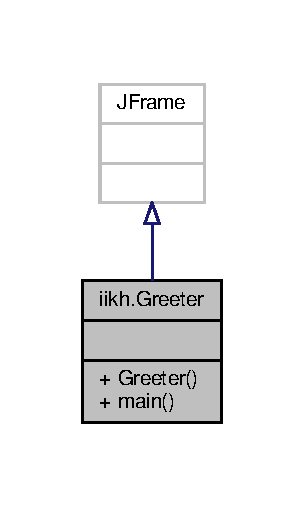
\includegraphics[width=146pt]{classiikh_1_1Greeter__inherit__graph}
\end{center}
\end{figure}


Collaboration diagram for iikh.\-Greeter\-:
\nopagebreak
\begin{figure}[H]
\begin{center}
\leavevmode
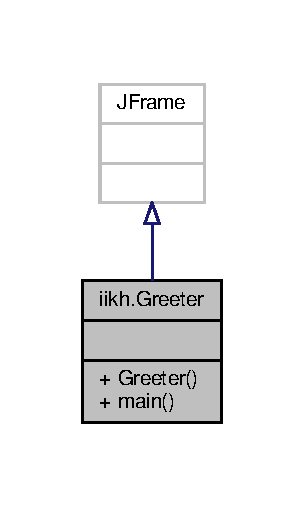
\includegraphics[width=146pt]{classiikh_1_1Greeter__coll__graph}
\end{center}
\end{figure}
\subsection*{Public Member Functions}
\begin{DoxyCompactItemize}
\item 
\hyperlink{classiikh_1_1Greeter_ac19a24071c8e4eca7214e2591b63df7c}{Greeter} ()
\end{DoxyCompactItemize}
\subsection*{Static Public Member Functions}
\begin{DoxyCompactItemize}
\item 
static void \hyperlink{classiikh_1_1Greeter_a8c6f110d372bfa6b7c807cb4d6dd57f0}{main} (String args\mbox{[}$\,$\mbox{]})
\end{DoxyCompactItemize}


\subsection{Detailed Description}
\begin{DoxyAuthor}{Author}
abhinav 
\end{DoxyAuthor}


\subsection{Constructor \& Destructor Documentation}
\hypertarget{classiikh_1_1Greeter_ac19a24071c8e4eca7214e2591b63df7c}{\index{iikh\-::\-Greeter@{iikh\-::\-Greeter}!Greeter@{Greeter}}
\index{Greeter@{Greeter}!iikh::Greeter@{iikh\-::\-Greeter}}
\subsubsection[{Greeter}]{\setlength{\rightskip}{0pt plus 5cm}iikh.\-Greeter.\-Greeter (
\begin{DoxyParamCaption}
{}
\end{DoxyParamCaption}
)\hspace{0.3cm}{\ttfamily [inline]}}}\label{classiikh_1_1Greeter_ac19a24071c8e4eca7214e2591b63df7c}
Creates new form \hyperlink{classiikh_1_1Greeter}{Greeter} 

\subsection{Member Function Documentation}
\hypertarget{classiikh_1_1Greeter_a8c6f110d372bfa6b7c807cb4d6dd57f0}{\index{iikh\-::\-Greeter@{iikh\-::\-Greeter}!main@{main}}
\index{main@{main}!iikh::Greeter@{iikh\-::\-Greeter}}
\subsubsection[{main}]{\setlength{\rightskip}{0pt plus 5cm}static void iikh.\-Greeter.\-main (
\begin{DoxyParamCaption}
\item[{String}]{args\mbox{[}$\,$\mbox{]}}
\end{DoxyParamCaption}
)\hspace{0.3cm}{\ttfamily [inline]}, {\ttfamily [static]}}}\label{classiikh_1_1Greeter_a8c6f110d372bfa6b7c807cb4d6dd57f0}

\begin{DoxyParams}{Parameters}
{\em args} & the command line arguments \\
\hline
\end{DoxyParams}


The documentation for this class was generated from the following file\-:\begin{DoxyCompactItemize}
\item 
\hyperlink{Greeter_8java}{Greeter.\-java}\end{DoxyCompactItemize}

\hypertarget{classiikh_1_1IIKH}{\section{iikh.\-I\-I\-K\-H Class Reference}
\label{classiikh_1_1IIKH}\index{iikh.\-I\-I\-K\-H@{iikh.\-I\-I\-K\-H}}
}


Collaboration diagram for iikh.\-I\-I\-K\-H\-:
\nopagebreak
\begin{figure}[H]
\begin{center}
\leavevmode
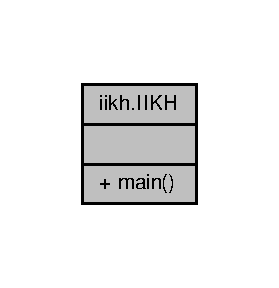
\includegraphics[width=134pt]{classiikh_1_1IIKH__coll__graph}
\end{center}
\end{figure}
\subsection*{Static Public Member Functions}
\begin{DoxyCompactItemize}
\item 
static void \hyperlink{classiikh_1_1IIKH_a2370515e48e464b157d4a5ce2dfd3332}{main} (String\mbox{[}$\,$\mbox{]} args)
\end{DoxyCompactItemize}


\subsection{Detailed Description}
\begin{DoxyAuthor}{Author}
user 
\end{DoxyAuthor}


\subsection{Member Function Documentation}
\hypertarget{classiikh_1_1IIKH_a2370515e48e464b157d4a5ce2dfd3332}{\index{iikh\-::\-I\-I\-K\-H@{iikh\-::\-I\-I\-K\-H}!main@{main}}
\index{main@{main}!iikh::IIKH@{iikh\-::\-I\-I\-K\-H}}
\subsubsection[{main}]{\setlength{\rightskip}{0pt plus 5cm}static void iikh.\-I\-I\-K\-H.\-main (
\begin{DoxyParamCaption}
\item[{String\mbox{[}$\,$\mbox{]}}]{args}
\end{DoxyParamCaption}
)\hspace{0.3cm}{\ttfamily [inline]}, {\ttfamily [static]}}}\label{classiikh_1_1IIKH_a2370515e48e464b157d4a5ce2dfd3332}

\begin{DoxyParams}{Parameters}
{\em args} & the command line arguments \\
\hline
\end{DoxyParams}


The documentation for this class was generated from the following file\-:\begin{DoxyCompactItemize}
\item 
\hyperlink{IIKH_8java}{I\-I\-K\-H.\-java}\end{DoxyCompactItemize}

\hypertarget{classiikh_1_1MealData}{\section{iikh.\-Meal\-Data Class Reference}
\label{classiikh_1_1MealData}\index{iikh.\-Meal\-Data@{iikh.\-Meal\-Data}}
}


Collaboration diagram for iikh.\-Meal\-Data\-:
\nopagebreak
\begin{figure}[H]
\begin{center}
\leavevmode
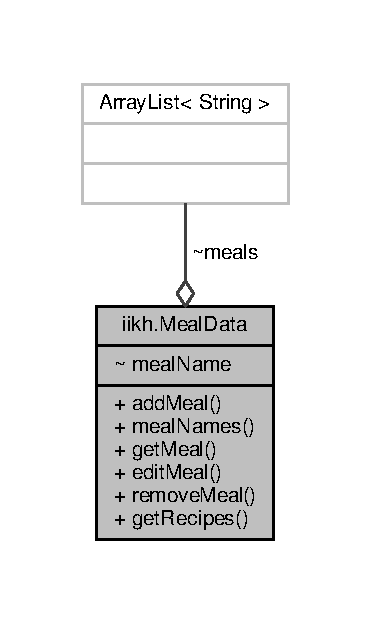
\includegraphics[width=178pt]{classiikh_1_1MealData__coll__graph}
\end{center}
\end{figure}
\subsection*{Public Member Functions}
\begin{DoxyCompactItemize}
\item 
void \hyperlink{classiikh_1_1MealData_a5e0c768c8948199c94fcd73b7b23b1ab}{add\-Meal} (String meal\-Name, Array\-List$<$ String $>$ recipes)
\item 
Array\-List$<$ String $>$ \hyperlink{classiikh_1_1MealData_a52bb34ef7c9131647e13cb540201b991}{meal\-Names} ()
\item 
void \hyperlink{classiikh_1_1MealData_a9cd185cb7c3d4e2bc42f4fdef2d5eab0}{get\-Meal} (String meal\-Name)
\item 
void \hyperlink{classiikh_1_1MealData_a7b7dd623490e5468cde17108ca4ef249}{edit\-Meal} (String oldmeal\-Name, String newmeal\-Name, Array\-List$<$ String $>$ recipes)
\item 
void \hyperlink{classiikh_1_1MealData_a4f8082d1c78009c2ac358d1a1e304f5b}{remove\-Meal} (String meal\-Name)
\item 
Array\-List$<$ String $>$ \hyperlink{classiikh_1_1MealData_a57e6f2b3be7ea592beac256bc92f89f2}{get\-Recipes} ()
\end{DoxyCompactItemize}


\subsection{Detailed Description}
\begin{DoxyAuthor}{Author}
abhinav 
\end{DoxyAuthor}


\subsection{Member Function Documentation}
\hypertarget{classiikh_1_1MealData_a5e0c768c8948199c94fcd73b7b23b1ab}{\index{iikh\-::\-Meal\-Data@{iikh\-::\-Meal\-Data}!add\-Meal@{add\-Meal}}
\index{add\-Meal@{add\-Meal}!iikh::MealData@{iikh\-::\-Meal\-Data}}
\subsubsection[{add\-Meal}]{\setlength{\rightskip}{0pt plus 5cm}void iikh.\-Meal\-Data.\-add\-Meal (
\begin{DoxyParamCaption}
\item[{String}]{meal\-Name, }
\item[{Array\-List$<$ String $>$}]{recipes}
\end{DoxyParamCaption}
)\hspace{0.3cm}{\ttfamily [inline]}}}\label{classiikh_1_1MealData_a5e0c768c8948199c94fcd73b7b23b1ab}
\hypertarget{classiikh_1_1MealData_a7b7dd623490e5468cde17108ca4ef249}{\index{iikh\-::\-Meal\-Data@{iikh\-::\-Meal\-Data}!edit\-Meal@{edit\-Meal}}
\index{edit\-Meal@{edit\-Meal}!iikh::MealData@{iikh\-::\-Meal\-Data}}
\subsubsection[{edit\-Meal}]{\setlength{\rightskip}{0pt plus 5cm}void iikh.\-Meal\-Data.\-edit\-Meal (
\begin{DoxyParamCaption}
\item[{String}]{oldmeal\-Name, }
\item[{String}]{newmeal\-Name, }
\item[{Array\-List$<$ String $>$}]{recipes}
\end{DoxyParamCaption}
)\hspace{0.3cm}{\ttfamily [inline]}}}\label{classiikh_1_1MealData_a7b7dd623490e5468cde17108ca4ef249}
\hypertarget{classiikh_1_1MealData_a9cd185cb7c3d4e2bc42f4fdef2d5eab0}{\index{iikh\-::\-Meal\-Data@{iikh\-::\-Meal\-Data}!get\-Meal@{get\-Meal}}
\index{get\-Meal@{get\-Meal}!iikh::MealData@{iikh\-::\-Meal\-Data}}
\subsubsection[{get\-Meal}]{\setlength{\rightskip}{0pt plus 5cm}void iikh.\-Meal\-Data.\-get\-Meal (
\begin{DoxyParamCaption}
\item[{String}]{meal\-Name}
\end{DoxyParamCaption}
)\hspace{0.3cm}{\ttfamily [inline]}}}\label{classiikh_1_1MealData_a9cd185cb7c3d4e2bc42f4fdef2d5eab0}
\hypertarget{classiikh_1_1MealData_a57e6f2b3be7ea592beac256bc92f89f2}{\index{iikh\-::\-Meal\-Data@{iikh\-::\-Meal\-Data}!get\-Recipes@{get\-Recipes}}
\index{get\-Recipes@{get\-Recipes}!iikh::MealData@{iikh\-::\-Meal\-Data}}
\subsubsection[{get\-Recipes}]{\setlength{\rightskip}{0pt plus 5cm}Array\-List$<$String$>$ iikh.\-Meal\-Data.\-get\-Recipes (
\begin{DoxyParamCaption}
{}
\end{DoxyParamCaption}
)\hspace{0.3cm}{\ttfamily [inline]}}}\label{classiikh_1_1MealData_a57e6f2b3be7ea592beac256bc92f89f2}
\hypertarget{classiikh_1_1MealData_a52bb34ef7c9131647e13cb540201b991}{\index{iikh\-::\-Meal\-Data@{iikh\-::\-Meal\-Data}!meal\-Names@{meal\-Names}}
\index{meal\-Names@{meal\-Names}!iikh::MealData@{iikh\-::\-Meal\-Data}}
\subsubsection[{meal\-Names}]{\setlength{\rightskip}{0pt plus 5cm}Array\-List$<$String$>$ iikh.\-Meal\-Data.\-meal\-Names (
\begin{DoxyParamCaption}
{}
\end{DoxyParamCaption}
)\hspace{0.3cm}{\ttfamily [inline]}}}\label{classiikh_1_1MealData_a52bb34ef7c9131647e13cb540201b991}
\hypertarget{classiikh_1_1MealData_a4f8082d1c78009c2ac358d1a1e304f5b}{\index{iikh\-::\-Meal\-Data@{iikh\-::\-Meal\-Data}!remove\-Meal@{remove\-Meal}}
\index{remove\-Meal@{remove\-Meal}!iikh::MealData@{iikh\-::\-Meal\-Data}}
\subsubsection[{remove\-Meal}]{\setlength{\rightskip}{0pt plus 5cm}void iikh.\-Meal\-Data.\-remove\-Meal (
\begin{DoxyParamCaption}
\item[{String}]{meal\-Name}
\end{DoxyParamCaption}
)\hspace{0.3cm}{\ttfamily [inline]}}}\label{classiikh_1_1MealData_a4f8082d1c78009c2ac358d1a1e304f5b}


The documentation for this class was generated from the following file\-:\begin{DoxyCompactItemize}
\item 
\hyperlink{MealData_8java}{Meal\-Data.\-java}\end{DoxyCompactItemize}

\hypertarget{classiikh_1_1MealManager}{\section{iikh.\-Meal\-Manager Class Reference}
\label{classiikh_1_1MealManager}\index{iikh.\-Meal\-Manager@{iikh.\-Meal\-Manager}}
}


Inheritance diagram for iikh.\-Meal\-Manager\-:
\nopagebreak
\begin{figure}[H]
\begin{center}
\leavevmode
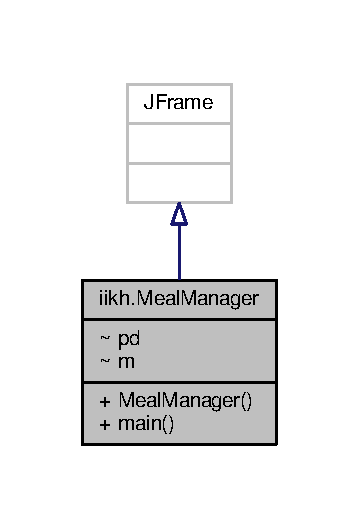
\includegraphics[width=172pt]{classiikh_1_1MealManager__inherit__graph}
\end{center}
\end{figure}


Collaboration diagram for iikh.\-Meal\-Manager\-:
\nopagebreak
\begin{figure}[H]
\begin{center}
\leavevmode
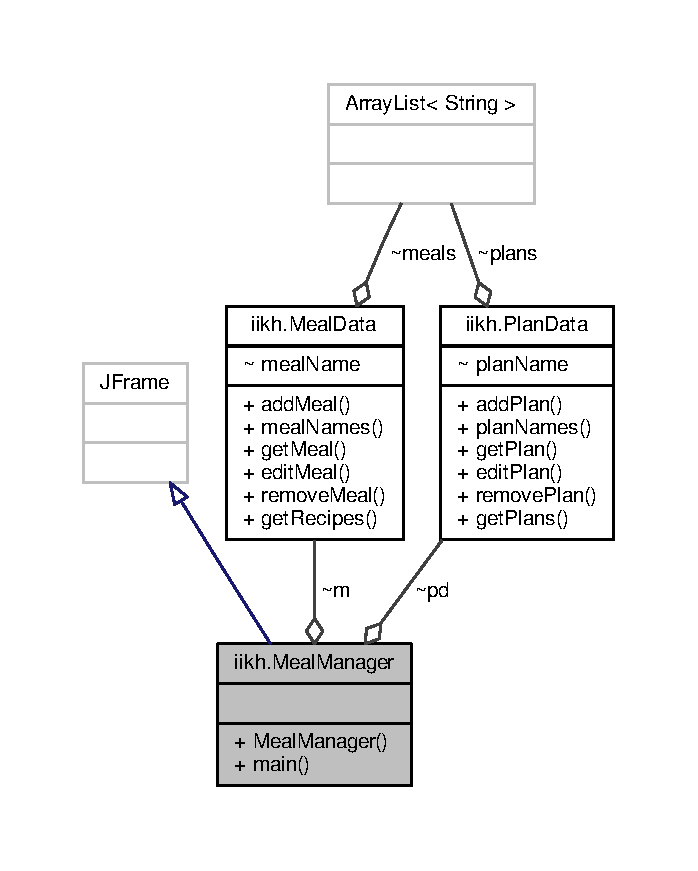
\includegraphics[width=335pt]{classiikh_1_1MealManager__coll__graph}
\end{center}
\end{figure}
\subsection*{Public Member Functions}
\begin{DoxyCompactItemize}
\item 
\hyperlink{classiikh_1_1MealManager_a8c04fa156bdf1b492f5fd020ff753e3b}{Meal\-Manager} ()
\end{DoxyCompactItemize}
\subsection*{Static Public Member Functions}
\begin{DoxyCompactItemize}
\item 
static void \hyperlink{classiikh_1_1MealManager_ad5d453d41fbfc9e4cefc08afef1465c5}{main} (String args\mbox{[}$\,$\mbox{]})
\end{DoxyCompactItemize}


\subsection{Detailed Description}
\begin{DoxyAuthor}{Author}
abhinav 
\end{DoxyAuthor}


\subsection{Constructor \& Destructor Documentation}
\hypertarget{classiikh_1_1MealManager_a8c04fa156bdf1b492f5fd020ff753e3b}{\index{iikh\-::\-Meal\-Manager@{iikh\-::\-Meal\-Manager}!Meal\-Manager@{Meal\-Manager}}
\index{Meal\-Manager@{Meal\-Manager}!iikh::MealManager@{iikh\-::\-Meal\-Manager}}
\subsubsection[{Meal\-Manager}]{\setlength{\rightskip}{0pt plus 5cm}iikh.\-Meal\-Manager.\-Meal\-Manager (
\begin{DoxyParamCaption}
{}
\end{DoxyParamCaption}
)\hspace{0.3cm}{\ttfamily [inline]}}}\label{classiikh_1_1MealManager_a8c04fa156bdf1b492f5fd020ff753e3b}


\subsection{Member Function Documentation}
\hypertarget{classiikh_1_1MealManager_ad5d453d41fbfc9e4cefc08afef1465c5}{\index{iikh\-::\-Meal\-Manager@{iikh\-::\-Meal\-Manager}!main@{main}}
\index{main@{main}!iikh::MealManager@{iikh\-::\-Meal\-Manager}}
\subsubsection[{main}]{\setlength{\rightskip}{0pt plus 5cm}static void iikh.\-Meal\-Manager.\-main (
\begin{DoxyParamCaption}
\item[{String}]{args\mbox{[}$\,$\mbox{]}}
\end{DoxyParamCaption}
)\hspace{0.3cm}{\ttfamily [inline]}, {\ttfamily [static]}}}\label{classiikh_1_1MealManager_ad5d453d41fbfc9e4cefc08afef1465c5}

\begin{DoxyParams}{Parameters}
{\em args} & the command line arguments \\
\hline
\end{DoxyParams}


The documentation for this class was generated from the following file\-:\begin{DoxyCompactItemize}
\item 
\hyperlink{MealManager_8java}{Meal\-Manager.\-java}\end{DoxyCompactItemize}

\hypertarget{classiikh_1_1PlanData}{\section{iikh.\-Plan\-Data Class Reference}
\label{classiikh_1_1PlanData}\index{iikh.\-Plan\-Data@{iikh.\-Plan\-Data}}
}


Collaboration diagram for iikh.\-Plan\-Data\-:
\nopagebreak
\begin{figure}[H]
\begin{center}
\leavevmode
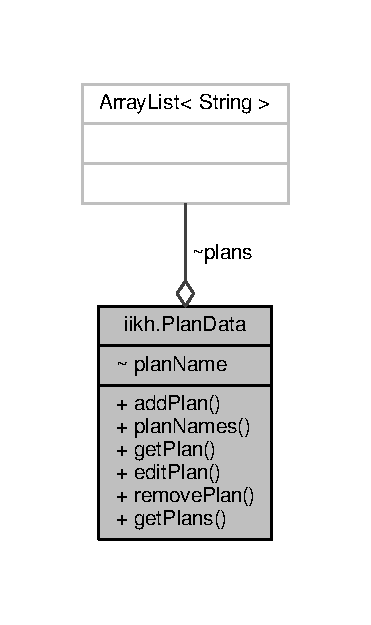
\includegraphics[width=178pt]{classiikh_1_1PlanData__coll__graph}
\end{center}
\end{figure}
\subsection*{Public Member Functions}
\begin{DoxyCompactItemize}
\item 
void \hyperlink{classiikh_1_1PlanData_a86e0a03aefaa8d01863abe280ccd67b2}{add\-Plan} (String plan\-Name, Array\-List$<$ String $>$ recipes)
\item 
Array\-List$<$ String $>$ \hyperlink{classiikh_1_1PlanData_a667ee00aa6c489febaea35301d623be8}{plan\-Names} ()
\item 
void \hyperlink{classiikh_1_1PlanData_a5b382a34fd5e7ea0f751cdf235ed7c58}{get\-Plan} (String plan\-Name)
\item 
void \hyperlink{classiikh_1_1PlanData_a3f6e92b4b5972aca919b10e27dd46ee1}{edit\-Plan} (String oldplan\-Name, String newplan\-Name, Array\-List$<$ String $>$ recipes)
\item 
void \hyperlink{classiikh_1_1PlanData_a3f2a629308fac33d893afff49131e931}{remove\-Plan} (String plan\-Name)
\item 
Array\-List$<$ String $>$ \hyperlink{classiikh_1_1PlanData_a979dec6192d46f34736fdd7eab84c532}{get\-Plans} ()
\end{DoxyCompactItemize}


\subsection{Detailed Description}
\begin{DoxyAuthor}{Author}
abhinav 
\end{DoxyAuthor}


\subsection{Member Function Documentation}
\hypertarget{classiikh_1_1PlanData_a86e0a03aefaa8d01863abe280ccd67b2}{\index{iikh\-::\-Plan\-Data@{iikh\-::\-Plan\-Data}!add\-Plan@{add\-Plan}}
\index{add\-Plan@{add\-Plan}!iikh::PlanData@{iikh\-::\-Plan\-Data}}
\subsubsection[{add\-Plan}]{\setlength{\rightskip}{0pt plus 5cm}void iikh.\-Plan\-Data.\-add\-Plan (
\begin{DoxyParamCaption}
\item[{String}]{plan\-Name, }
\item[{Array\-List$<$ String $>$}]{recipes}
\end{DoxyParamCaption}
)\hspace{0.3cm}{\ttfamily [inline]}}}\label{classiikh_1_1PlanData_a86e0a03aefaa8d01863abe280ccd67b2}
\hypertarget{classiikh_1_1PlanData_a3f6e92b4b5972aca919b10e27dd46ee1}{\index{iikh\-::\-Plan\-Data@{iikh\-::\-Plan\-Data}!edit\-Plan@{edit\-Plan}}
\index{edit\-Plan@{edit\-Plan}!iikh::PlanData@{iikh\-::\-Plan\-Data}}
\subsubsection[{edit\-Plan}]{\setlength{\rightskip}{0pt plus 5cm}void iikh.\-Plan\-Data.\-edit\-Plan (
\begin{DoxyParamCaption}
\item[{String}]{oldplan\-Name, }
\item[{String}]{newplan\-Name, }
\item[{Array\-List$<$ String $>$}]{recipes}
\end{DoxyParamCaption}
)\hspace{0.3cm}{\ttfamily [inline]}}}\label{classiikh_1_1PlanData_a3f6e92b4b5972aca919b10e27dd46ee1}
\hypertarget{classiikh_1_1PlanData_a5b382a34fd5e7ea0f751cdf235ed7c58}{\index{iikh\-::\-Plan\-Data@{iikh\-::\-Plan\-Data}!get\-Plan@{get\-Plan}}
\index{get\-Plan@{get\-Plan}!iikh::PlanData@{iikh\-::\-Plan\-Data}}
\subsubsection[{get\-Plan}]{\setlength{\rightskip}{0pt plus 5cm}void iikh.\-Plan\-Data.\-get\-Plan (
\begin{DoxyParamCaption}
\item[{String}]{plan\-Name}
\end{DoxyParamCaption}
)\hspace{0.3cm}{\ttfamily [inline]}}}\label{classiikh_1_1PlanData_a5b382a34fd5e7ea0f751cdf235ed7c58}
\hypertarget{classiikh_1_1PlanData_a979dec6192d46f34736fdd7eab84c532}{\index{iikh\-::\-Plan\-Data@{iikh\-::\-Plan\-Data}!get\-Plans@{get\-Plans}}
\index{get\-Plans@{get\-Plans}!iikh::PlanData@{iikh\-::\-Plan\-Data}}
\subsubsection[{get\-Plans}]{\setlength{\rightskip}{0pt plus 5cm}Array\-List$<$String$>$ iikh.\-Plan\-Data.\-get\-Plans (
\begin{DoxyParamCaption}
{}
\end{DoxyParamCaption}
)\hspace{0.3cm}{\ttfamily [inline]}}}\label{classiikh_1_1PlanData_a979dec6192d46f34736fdd7eab84c532}
\hypertarget{classiikh_1_1PlanData_a667ee00aa6c489febaea35301d623be8}{\index{iikh\-::\-Plan\-Data@{iikh\-::\-Plan\-Data}!plan\-Names@{plan\-Names}}
\index{plan\-Names@{plan\-Names}!iikh::PlanData@{iikh\-::\-Plan\-Data}}
\subsubsection[{plan\-Names}]{\setlength{\rightskip}{0pt plus 5cm}Array\-List$<$String$>$ iikh.\-Plan\-Data.\-plan\-Names (
\begin{DoxyParamCaption}
{}
\end{DoxyParamCaption}
)\hspace{0.3cm}{\ttfamily [inline]}}}\label{classiikh_1_1PlanData_a667ee00aa6c489febaea35301d623be8}
\hypertarget{classiikh_1_1PlanData_a3f2a629308fac33d893afff49131e931}{\index{iikh\-::\-Plan\-Data@{iikh\-::\-Plan\-Data}!remove\-Plan@{remove\-Plan}}
\index{remove\-Plan@{remove\-Plan}!iikh::PlanData@{iikh\-::\-Plan\-Data}}
\subsubsection[{remove\-Plan}]{\setlength{\rightskip}{0pt plus 5cm}void iikh.\-Plan\-Data.\-remove\-Plan (
\begin{DoxyParamCaption}
\item[{String}]{plan\-Name}
\end{DoxyParamCaption}
)\hspace{0.3cm}{\ttfamily [inline]}}}\label{classiikh_1_1PlanData_a3f2a629308fac33d893afff49131e931}


The documentation for this class was generated from the following file\-:\begin{DoxyCompactItemize}
\item 
\hyperlink{PlanData_8java}{Plan\-Data.\-java}\end{DoxyCompactItemize}

\hypertarget{classiikh_1_1PlanManager}{\section{iikh.\-Plan\-Manager Class Reference}
\label{classiikh_1_1PlanManager}\index{iikh.\-Plan\-Manager@{iikh.\-Plan\-Manager}}
}


Inheritance diagram for iikh.\-Plan\-Manager\-:
\nopagebreak
\begin{figure}[H]
\begin{center}
\leavevmode
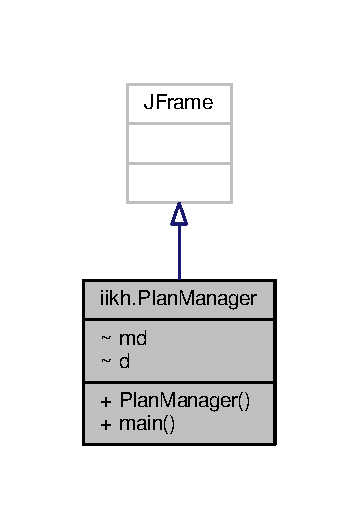
\includegraphics[width=172pt]{classiikh_1_1PlanManager__inherit__graph}
\end{center}
\end{figure}


Collaboration diagram for iikh.\-Plan\-Manager\-:
\nopagebreak
\begin{figure}[H]
\begin{center}
\leavevmode
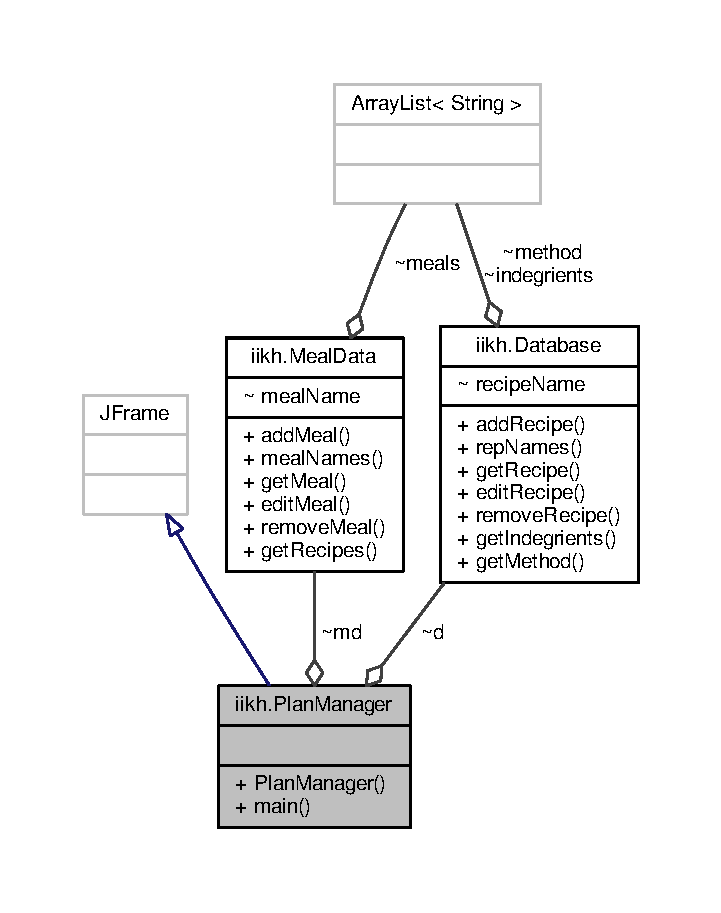
\includegraphics[width=346pt]{classiikh_1_1PlanManager__coll__graph}
\end{center}
\end{figure}
\subsection*{Public Member Functions}
\begin{DoxyCompactItemize}
\item 
\hyperlink{classiikh_1_1PlanManager_aea91e5e77b8fb5a20c3d8d383692b7d4}{Plan\-Manager} ()
\end{DoxyCompactItemize}
\subsection*{Static Public Member Functions}
\begin{DoxyCompactItemize}
\item 
static void \hyperlink{classiikh_1_1PlanManager_ae9f6edba1648bd9f9975b959daf9429d}{main} (String args\mbox{[}$\,$\mbox{]})
\end{DoxyCompactItemize}


\subsection{Detailed Description}
\begin{DoxyAuthor}{Author}
abhinav 
\end{DoxyAuthor}


\subsection{Constructor \& Destructor Documentation}
\hypertarget{classiikh_1_1PlanManager_aea91e5e77b8fb5a20c3d8d383692b7d4}{\index{iikh\-::\-Plan\-Manager@{iikh\-::\-Plan\-Manager}!Plan\-Manager@{Plan\-Manager}}
\index{Plan\-Manager@{Plan\-Manager}!iikh::PlanManager@{iikh\-::\-Plan\-Manager}}
\subsubsection[{Plan\-Manager}]{\setlength{\rightskip}{0pt plus 5cm}iikh.\-Plan\-Manager.\-Plan\-Manager (
\begin{DoxyParamCaption}
{}
\end{DoxyParamCaption}
)\hspace{0.3cm}{\ttfamily [inline]}}}\label{classiikh_1_1PlanManager_aea91e5e77b8fb5a20c3d8d383692b7d4}


\subsection{Member Function Documentation}
\hypertarget{classiikh_1_1PlanManager_ae9f6edba1648bd9f9975b959daf9429d}{\index{iikh\-::\-Plan\-Manager@{iikh\-::\-Plan\-Manager}!main@{main}}
\index{main@{main}!iikh::PlanManager@{iikh\-::\-Plan\-Manager}}
\subsubsection[{main}]{\setlength{\rightskip}{0pt plus 5cm}static void iikh.\-Plan\-Manager.\-main (
\begin{DoxyParamCaption}
\item[{String}]{args\mbox{[}$\,$\mbox{]}}
\end{DoxyParamCaption}
)\hspace{0.3cm}{\ttfamily [inline]}, {\ttfamily [static]}}}\label{classiikh_1_1PlanManager_ae9f6edba1648bd9f9975b959daf9429d}

\begin{DoxyParams}{Parameters}
{\em args} & the command line arguments \\
\hline
\end{DoxyParams}


The documentation for this class was generated from the following file\-:\begin{DoxyCompactItemize}
\item 
\hyperlink{PlanManager_8java}{Plan\-Manager.\-java}\end{DoxyCompactItemize}

\hypertarget{classiikh_1_1RecipeForm}{\section{iikh.\-Recipe\-Form Class Reference}
\label{classiikh_1_1RecipeForm}\index{iikh.\-Recipe\-Form@{iikh.\-Recipe\-Form}}
}


Inheritance diagram for iikh.\-Recipe\-Form\-:
\nopagebreak
\begin{figure}[H]
\begin{center}
\leavevmode
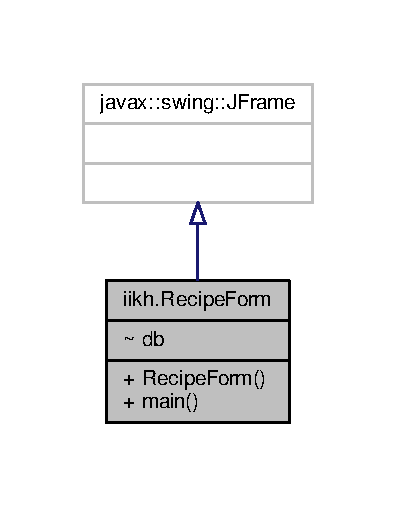
\includegraphics[width=190pt]{classiikh_1_1RecipeForm__inherit__graph}
\end{center}
\end{figure}


Collaboration diagram for iikh.\-Recipe\-Form\-:
\nopagebreak
\begin{figure}[H]
\begin{center}
\leavevmode
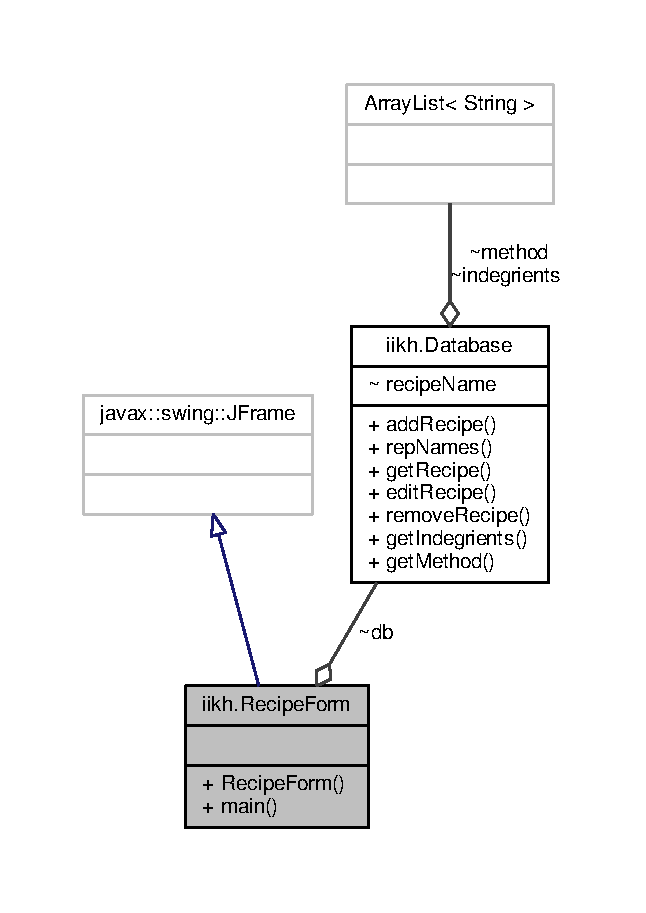
\includegraphics[width=310pt]{classiikh_1_1RecipeForm__coll__graph}
\end{center}
\end{figure}
\subsection*{Public Member Functions}
\begin{DoxyCompactItemize}
\item 
\hyperlink{classiikh_1_1RecipeForm_a0f56916cccfce4153ab9a8094106782c}{Recipe\-Form} ()
\end{DoxyCompactItemize}
\subsection*{Static Public Member Functions}
\begin{DoxyCompactItemize}
\item 
static void \hyperlink{classiikh_1_1RecipeForm_a0a981165c0940c57543345eb4c0803d2}{main} (String args\mbox{[}$\,$\mbox{]})
\end{DoxyCompactItemize}


\subsection{Detailed Description}
\begin{DoxyAuthor}{Author}
abhinav 
\end{DoxyAuthor}


\subsection{Constructor \& Destructor Documentation}
\hypertarget{classiikh_1_1RecipeForm_a0f56916cccfce4153ab9a8094106782c}{\index{iikh\-::\-Recipe\-Form@{iikh\-::\-Recipe\-Form}!Recipe\-Form@{Recipe\-Form}}
\index{Recipe\-Form@{Recipe\-Form}!iikh::RecipeForm@{iikh\-::\-Recipe\-Form}}
\subsubsection[{Recipe\-Form}]{\setlength{\rightskip}{0pt plus 5cm}iikh.\-Recipe\-Form.\-Recipe\-Form (
\begin{DoxyParamCaption}
{}
\end{DoxyParamCaption}
)\hspace{0.3cm}{\ttfamily [inline]}}}\label{classiikh_1_1RecipeForm_a0f56916cccfce4153ab9a8094106782c}


\subsection{Member Function Documentation}
\hypertarget{classiikh_1_1RecipeForm_a0a981165c0940c57543345eb4c0803d2}{\index{iikh\-::\-Recipe\-Form@{iikh\-::\-Recipe\-Form}!main@{main}}
\index{main@{main}!iikh::RecipeForm@{iikh\-::\-Recipe\-Form}}
\subsubsection[{main}]{\setlength{\rightskip}{0pt plus 5cm}static void iikh.\-Recipe\-Form.\-main (
\begin{DoxyParamCaption}
\item[{String}]{args\mbox{[}$\,$\mbox{]}}
\end{DoxyParamCaption}
)\hspace{0.3cm}{\ttfamily [inline]}, {\ttfamily [static]}}}\label{classiikh_1_1RecipeForm_a0a981165c0940c57543345eb4c0803d2}

\begin{DoxyParams}{Parameters}
{\em args} & the command line arguments \\
\hline
\end{DoxyParams}


The documentation for this class was generated from the following file\-:\begin{DoxyCompactItemize}
\item 
\hyperlink{RecipeForm_8java}{Recipe\-Form.\-java}\end{DoxyCompactItemize}

\chapter{File Documentation}
\hypertarget{Database_8java}{\section{Database.\-java File Reference}
\label{Database_8java}\index{Database.\-java@{Database.\-java}}
}
\subsection*{Classes}
\begin{DoxyCompactItemize}
\item 
class \hyperlink{classiikh_1_1Database}{iikh.\-Database}
\end{DoxyCompactItemize}
\subsection*{Packages}
\begin{DoxyCompactItemize}
\item 
package \hyperlink{namespaceiikh}{iikh}
\end{DoxyCompactItemize}

\hypertarget{Greeter_8java}{\section{Greeter.\-java File Reference}
\label{Greeter_8java}\index{Greeter.\-java@{Greeter.\-java}}
}
\subsection*{Classes}
\begin{DoxyCompactItemize}
\item 
class \hyperlink{classcarcruisecontrolsystem_1_1Greeter}{carcruisecontrolsystem.\-Greeter}
\end{DoxyCompactItemize}
\subsection*{Packages}
\begin{DoxyCompactItemize}
\item 
package \hyperlink{namespacecarcruisecontrolsystem}{carcruisecontrolsystem}
\end{DoxyCompactItemize}

\hypertarget{IIKH_8java}{\section{I\-I\-K\-H.\-java File Reference}
\label{IIKH_8java}\index{I\-I\-K\-H.\-java@{I\-I\-K\-H.\-java}}
}
\subsection*{Classes}
\begin{DoxyCompactItemize}
\item 
class \hyperlink{classiikh_1_1IIKH}{iikh.\-I\-I\-K\-H}
\end{DoxyCompactItemize}
\subsection*{Packages}
\begin{DoxyCompactItemize}
\item 
package \hyperlink{namespaceiikh}{iikh}
\end{DoxyCompactItemize}

\hypertarget{MealData_8java}{\section{Meal\-Data.\-java File Reference}
\label{MealData_8java}\index{Meal\-Data.\-java@{Meal\-Data.\-java}}
}
\subsection*{Classes}
\begin{DoxyCompactItemize}
\item 
class \hyperlink{classiikh_1_1MealData}{iikh.\-Meal\-Data}
\end{DoxyCompactItemize}
\subsection*{Packages}
\begin{DoxyCompactItemize}
\item 
package \hyperlink{namespaceiikh}{iikh}
\end{DoxyCompactItemize}

\hypertarget{MealManager_8java}{\section{Meal\-Manager.\-java File Reference}
\label{MealManager_8java}\index{Meal\-Manager.\-java@{Meal\-Manager.\-java}}
}
\subsection*{Classes}
\begin{DoxyCompactItemize}
\item 
class \hyperlink{classiikh_1_1MealManager}{iikh.\-Meal\-Manager}
\end{DoxyCompactItemize}
\subsection*{Packages}
\begin{DoxyCompactItemize}
\item 
package \hyperlink{namespaceiikh}{iikh}
\end{DoxyCompactItemize}

\hypertarget{PlanData_8java}{\section{Plan\-Data.\-java File Reference}
\label{PlanData_8java}\index{Plan\-Data.\-java@{Plan\-Data.\-java}}
}
\subsection*{Classes}
\begin{DoxyCompactItemize}
\item 
class \hyperlink{classiikh_1_1PlanData}{iikh.\-Plan\-Data}
\end{DoxyCompactItemize}
\subsection*{Packages}
\begin{DoxyCompactItemize}
\item 
package \hyperlink{namespaceiikh}{iikh}
\end{DoxyCompactItemize}

\hypertarget{PlanManager_8java}{\section{Plan\-Manager.\-java File Reference}
\label{PlanManager_8java}\index{Plan\-Manager.\-java@{Plan\-Manager.\-java}}
}
\subsection*{Classes}
\begin{DoxyCompactItemize}
\item 
class \hyperlink{classiikh_1_1PlanManager}{iikh.\-Plan\-Manager}
\end{DoxyCompactItemize}
\subsection*{Packages}
\begin{DoxyCompactItemize}
\item 
package \hyperlink{namespaceiikh}{iikh}
\end{DoxyCompactItemize}

\hypertarget{RecipeForm_8java}{\section{Recipe\-Form.\-java File Reference}
\label{RecipeForm_8java}\index{Recipe\-Form.\-java@{Recipe\-Form.\-java}}
}
\subsection*{Classes}
\begin{DoxyCompactItemize}
\item 
class \hyperlink{classiikh_1_1RecipeForm}{iikh.\-Recipe\-Form}
\end{DoxyCompactItemize}
\subsection*{Packages}
\begin{DoxyCompactItemize}
\item 
package \hyperlink{namespaceiikh}{iikh}
\end{DoxyCompactItemize}

%--- End generated contents ---

% Index
\newpage
\phantomsection
\addcontentsline{toc}{chapter}{Index}
\printindex

\end{document}
